\section{Exercise 5}

Consider the Quake III Arena Network Protocol, a stateless client-server protocol used by the classic multi-player game. 
Quake III supports multiple name servers (indeed, anyone can run their server, expose it to the whole Internet, and even have it indexed by the “master server” for easy discovery).
When a client connects to one of the many available servers, it needs to retrieve some information. 
To this purpose, the Quake III protocol implements the command gestatus, accessible without authentication.
When the server receives this command (via an UDP packet, destination port 27960), it replies with various information, such as: the list of enabled options, the hostname, the number of connected clients, and the type of supported game.

The image below is an example of protocol exchange, as shown in Wireshark, a packet capture tool: a client (192.168.1.39) sends a getstatus message to a server (128.66.0.59); the server replies with a statusResponse message, containing the information about the server in its payload.
\begin{figure}[H]
    \centering
    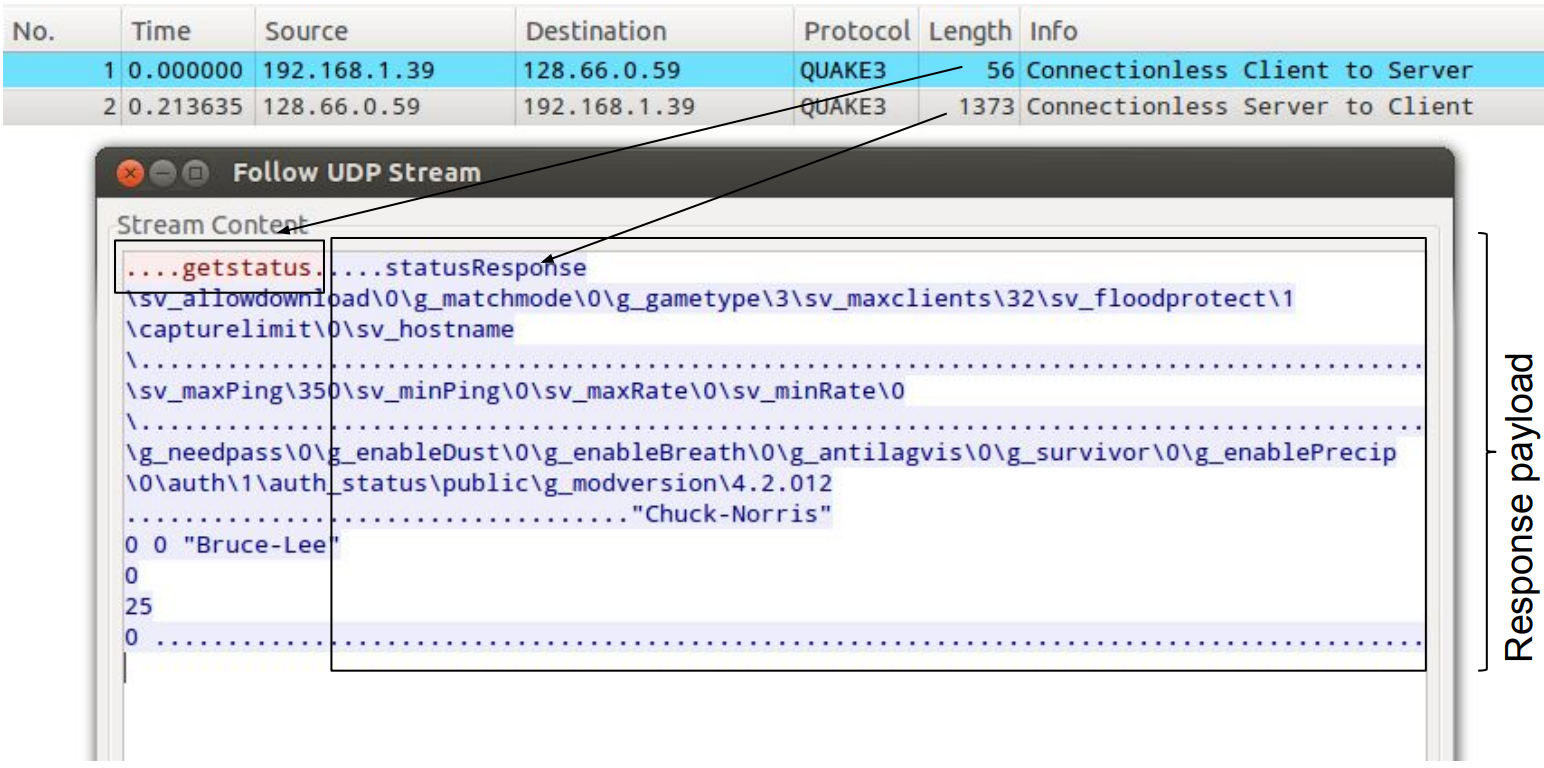
\includegraphics[width=0.75\linewidth]{images/net2.png}
\end{figure}

\begin{enumerate}
    \item The part of the Quake III Arena protocol described in the previous page can be misused to ease a DoS attack against a victim. 
        Please explain how an attack can misuse this protocol for this purpose, showing a concrete scenario where an attacker (who controls the server with IP address 93.184.216.32) aims to launch a DoS against the IP address 131.175.14.19. 
        Make sure you mention in your answer the feature of this protocol that allows the misuse for DoS purpose.
\end{enumerate}
We discovered in the wild a DoS attack that exploits this protocol. 
The network administrators of the company that was hit by this attack were able to capture the following headers of some suspect packets at their network's border firewall:
\begin{itemize}
    \item IP 87.98.244.20 (src port 27960) > 104.28.1.1 (dst port 12345) UDP, length 1373
    \item IP 87.98.244.20 (src port 27960) > 104.28.1.1 (dst port 12345) UDP, length 1373
    \item IP 188.138.125.254 (src port 27960) > 104.28.1.1 (dst port 32451) UDP, length 1400
    \item IP 188.138.125.254 (src port 27960) > 104.28.1.1 (dst port 32451) UDP, length 1400
    \item IP 188.138.125.254 (src port 27960) > 104.28.1.1 (dst port 32451) UDP, length 1400
    \item IP 188.138.125.254 (src port 27960) > 104.28.1.1 (dst port 32451) UDP, length 1400
    \item IP 188.138.125.254 (src port 27960) > 104.28.1.1 (dst port 32451) UDP, length 1400
    \item IP 5.196.85.159 (src port 27960) > 104.28.1.1 (dst port 32451) UDP, length 978
\end{itemize}
\begin{enumerate}
    \item [2. ] Can you identify the attacker's IP address? And the victim's one? Why?
    \item [3. ] As the network security administrator for the network hit by this attack (i.e., you control the border firewall and can add arbitrary rules), can you mitigate the effect of this attack or prevent it altogether? Why?
    \item [4. ] Consider the following mitigation implemented by the Quake III Arena server: when an IP address sends a getstatus command, the server will check if sender IP address has exceeded a pre-defined rate limit of 10 commands in a period of one second; if the rate limit is exceeded, the IP address is banned from the server forever.
    I   s this solution effective to mitigate the impact of the DoS scenario in the above attack? Why?
    \item [5. ] As the author(s) of Quake III Arena, you want to change the protocol to remove completely the issue that allows it from being exploited for DoS attacks. 
        How would you change the protocol to achieve this goal?
\end{enumerate}

\subsection*{Solution}
\begin{enumerate}
    \item The protocol allows an amplification-based denial of service: in fact, it is a UDP-based protocol, where a request of length 56 triggers a response of 1373 (in the example above), leading to a bandwidth amplification factor (BAF) of 24, i.e., amplifying the attacker's bandwidth of a factor of 24 (which means that, extremely roughly, if the attacker has a 100 Mbps network, given enough open Quake III servers with enough bandwidth each, it can flood the victim with a 2400 Mbps traffic).
        Concretely, the attacker (given he is in a network that allows IP spoofing) looks on the Internet for N open Quake III servers. 
        It spoofs the victim's IP address, and sends to such servers M UDP getstatus packets. 
        Each server will reply, for each packet received, with with the (long) information packet but, as  the source IP is spoofed, the M * N packets will go to the victim, instead of the attacker
    \item Attacker: no, the IP address you see in the logs are the ones of the vulnerable Quake III servers, not of the victim. 
        Also, the vulnerable Quake servers can't identify the attacker's IP address as they're spoofed with the victim's IP.
        Victim: yes, it's 104.28.1.1 (actually it could also be the border firewall or, in general, the company's network). 
    \item No. 
        Due of the amplifying properties of the protocol, if the attacker has enough bandwidth that, amplified by the 24x factor of the protocol, is greater or equal than the victim's bandwidth, the attacker always succeeds.
        However, if in this specific scenario the victim is the specific machine 104.28.1.1 and the bottleneck is not given by the network bandwidth of the Internet so company link, but from something else (e.g., the bandwidth of an internal network link, the capabilities of the machine itself, the capabilities of some network middlebox) implementing a firewall rule to drop UDP packet from source port 27960 can mitigate the attack (and thus it would be a good idea to implement).
        In general, though, a more powerful DoS attack may be launched to defeat this mitigation.
    \item No. 
        While this mitigation restricts an attacker to exploit a vulnerable server as an amplifier at most 10 packets per second (i.e., 13730 bytes/s, i.e., about 100 kbps), given that enough vulnerable servers are available the attacker can just use multiple vulnerable Quake III servers at once to defeat the rate limit.
        Moreover, if the attacker is targeting a network and not a specific IP address, it can spoof multiple IP of the same network, defeating the rate limiting.
    \item Solution 1: Implement an handshake at the UDP protocol level (making sure it does not have amplifying capabilities). 
        E.g., the client sends getinfo, the server responds with a nonce, and the client sends the nonce back to the server, then the server sends the long information message.
        Solution 2: Move the protocol to TCP instead of UDP as a transport protocol. 
        Due to the three-way handshake, TCP is immune to the amplification issue.
\end{enumerate}